\documentclass[tikz,border=5pt]{standalone}
\usepackage[T1]{fontenc}
\usepackage{amsmath}
\usetikzlibrary{arrows.meta,calc}

\definecolor{ink}{HTML}{1F2937}
\definecolor{slate}{HTML}{334155}
\definecolor{inputfill}{HTML}{EAF3FB}
\definecolor{inputedge}{HTML}{829DB4}
\definecolor{baselinefill}{HTML}{EEF2F6}
\definecolor{baselineedge}{HTML}{8795A5}
\definecolor{residualfill}{HTML}{FFF3DA}
\definecolor{residualedge}{HTML}{B49B63}
\definecolor{tealfill}{HTML}{E7F3EF}
\definecolor{tealedge}{HTML}{6B9D92}
\definecolor{tealarrow}{HTML}{227C70}
\definecolor{evalfill}{HTML}{F1EFF6}
\definecolor{evaledge}{HTML}{9892A5}
\definecolor{notegray}{HTML}{4B5563}

\newcommand{\mathblock}[1]{%
  {\fontsize{10.5}{13}\selectfont\(\displaystyle #1\)}%
}

% Including the standalone border, the page is 18 cm by 10.125 cm.
\newlength{\canvaswidth}
\newlength{\canvasheight}
\setlength{\canvaswidth}{\dimexpr18cm-10pt\relax}
\setlength{\canvasheight}{\dimexpr10.125cm-10pt\relax}

\begin{document}
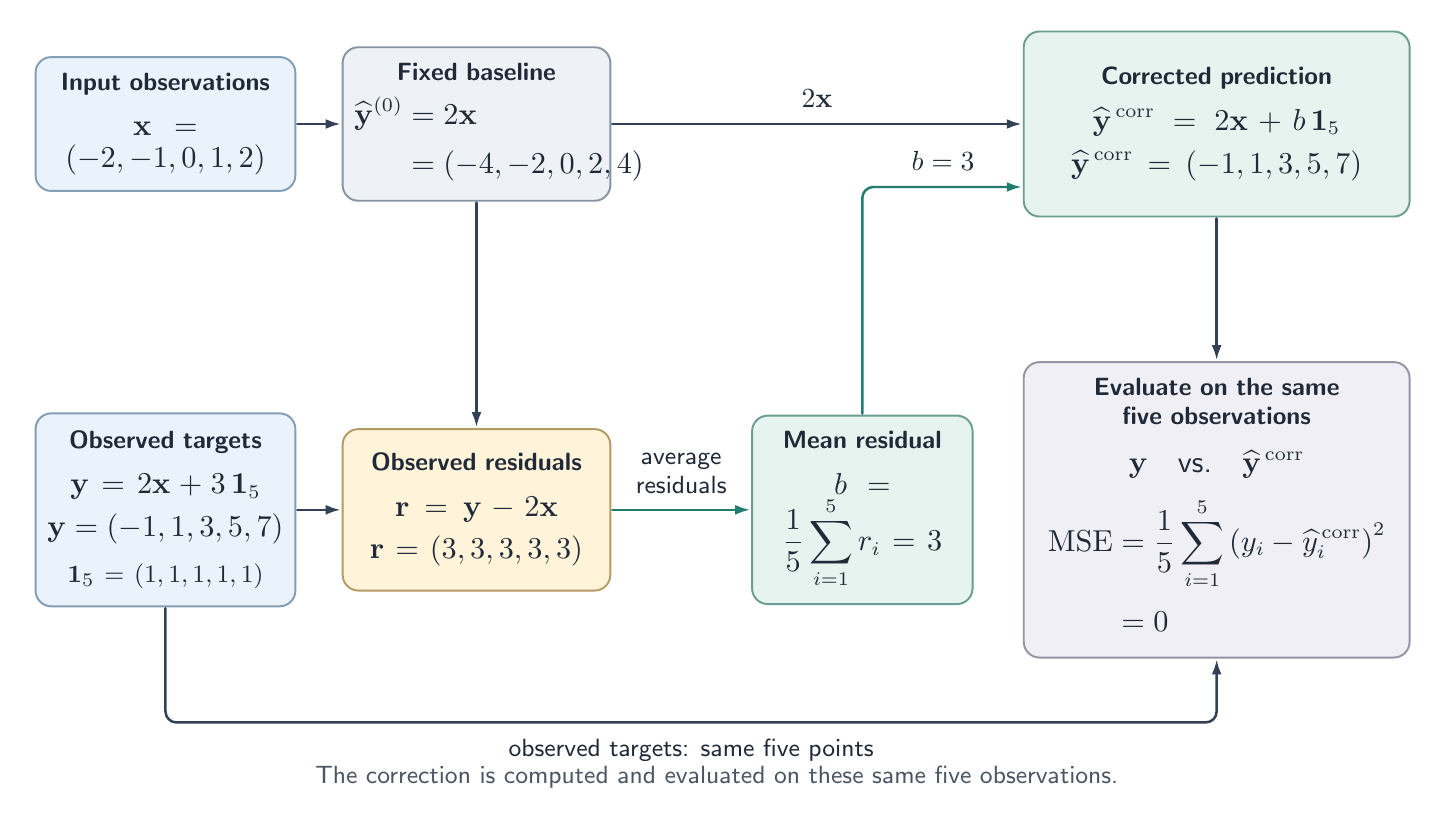
\begin{tikzpicture}[
  x=1cm,
  y=1cm,
  font=\sffamily\fontsize{9.5}{11.5}\selectfont,
  text=ink,
  box/.style={
    rectangle,
    rounded corners=2mm,
    line width=0.7pt,
    align=center,
    inner xsep=1.5mm,
    inner ysep=2mm,
    outer sep=0pt
  },
  supplied/.style={
    box,
    fill=inputfill,
    draw=inputedge,
    minimum width=3.3cm,
    text width=3.0cm
  },
  baseline/.style={
    box,
    fill=baselinefill,
    draw=baselineedge,
    minimum width=3.4cm,
    text width=3.1cm
  },
  residual/.style={
    box,
    fill=residualfill,
    draw=residualedge,
    minimum width=3.4cm,
    text width=3.1cm
  },
  mean/.style={
    box,
    fill=tealfill,
    draw=tealedge,
    minimum width=2.8cm,
    text width=2.5cm
  },
  corrected/.style={
    box,
    fill=tealfill,
    draw=tealedge,
    minimum width=4.9cm,
    text width=4.6cm
  },
  evaluation/.style={
    box,
    fill=evalfill,
    draw=evaledge,
    minimum width=4.9cm,
    text width=4.6cm
  },
  dependency/.style={
    draw=slate,
    line width=0.9pt,
    -{Latex[length=1.9mm,width=1.25mm]},
    shorten <=0.7pt,
    shorten >=0.7pt,
    line cap=round,
    line join=round
  },
  correction dependency/.style={
    dependency,
    draw=tealarrow
  },
  arrow label/.style={
    font=\sffamily\fontsize{9}{10.5}\selectfont,
    text=ink,
    fill=white,
    inner xsep=1pt,
    inner ysep=0.8pt,
    outer sep=0pt,
    align=center
  }
]

\fill[white] (0,0) rectangle (\canvaswidth,\canvasheight);

% Upper row.
\node[supplied, minimum height=1.65cm]
  (input) at (1.75,8.55) {
    \textbf{Input observations}\\[5pt]
    \mathblock{\mathbf{x}=(-2,-1,0,1,2)}
  };

\node[baseline, minimum height=1.95cm]
  (baseline) at (5.70,8.55) {
    \textbf{Fixed baseline}\\[5pt]
    \mathblock{
      \begin{aligned}
        \widehat{\mathbf{y}}^{(0)} &= 2\mathbf{x}\\[2pt]
                                 &= (-4,-2,0,2,4)
      \end{aligned}
    }
  };

\node[corrected, minimum height=2.35cm]
  (corrected) at (15.10,8.55) {
    \textbf{Corrected prediction}\\[5pt]
    \mathblock{
      \widehat{\mathbf{y}}^{\,\mathrm{corr}}
      =2\mathbf{x}+b\,\mathbf{1}_5
    }\\[4pt]
    \mathblock{
      \widehat{\mathbf{y}}^{\,\mathrm{corr}}
      =(-1,1,3,5,7)
    }
  };

% Lower row: all four node centers share the same horizontal axis.
\node[supplied, minimum height=2.45cm]
  (targets) at (1.75,3.65) {
    \textbf{Observed targets}\\[5pt]
    \mathblock{\mathbf{y}=2\mathbf{x}+3\,\mathbf{1}_5}\\[4pt]
    \mathblock{\mathbf{y}=(-1,1,3,5,7)}\\[5pt]
    {\fontsize{9.5}{11.5}\selectfont
      \(\mathbf{1}_5=(1,1,1,1,1)\)}
  };

\node[residual, minimum height=2.05cm]
  (residual) at (5.70,3.65) {
    \textbf{Observed residuals}\\[5pt]
    \mathblock{\mathbf{r}=\mathbf{y}-2\mathbf{x}}\\[4pt]
    \mathblock{\mathbf{r}=(3,3,3,3,3)}
  };

\node[mean, minimum height=1.80cm]
  (mean) at (10.60,3.65) {
    \textbf{Mean residual}\\[5pt]
    \mathblock{b=\frac{1}{5}\sum_{i=1}^{5}r_i=3}
  };

\node[evaluation, minimum height=3.45cm]
  (evaluation) at (15.10,3.65) {
    \textbf{Evaluate on the same}\\[-1pt]
    \textbf{five observations}\\[6pt]
    \mathblock{
      \mathbf{y}\quad\text{vs.}\quad
      \widehat{\mathbf{y}}^{\,\mathrm{corr}}
    }\\[6pt]
    \mathblock{
      \begin{aligned}
        \mathrm{MSE}
          &=\frac{1}{5}\sum_{i=1}^{5}
            \left(y_i-\widehat y_i^{\,\mathrm{corr}}\right)^2\\[2pt]
          &=0
      \end{aligned}
    }
  };

% 1. Input observations to fixed baseline.
\draw[dependency] (input.east) -- (baseline.west);

% 2. Fixed baseline to observed residuals.
\draw[dependency] (baseline.south) -- (residual.north);

% 3. Observed targets to observed residuals.
\draw[dependency] (targets.east) -- (residual.west);

% 4. Observed residuals to their scalar mean.
\draw[correction dependency]
  (residual.east) --
  node[arrow label, above=1.8mm]
    {average\\residuals}
  (mean.west);

% 5. Baseline contribution to corrected prediction.
\draw[dependency]
  (baseline.east) --
  node[arrow label, above=1.8mm]
    {\fontsize{10}{12}\selectfont\(2\mathbf{x}\)}
  (corrected.west);

% 6. Scalar correction enters a separate, lower left-edge port.
\coordinate (correction elbow) at (10.60,7.75);
\coordinate (correction port) at ([yshift=-8mm]corrected.west);
\draw[correction dependency, rounded corners=1.4mm]
  (mean.north) --
  (correction elbow) --
  node[arrow label, above=1.8mm]
    {\fontsize{10}{12}\selectfont\(b=3\)}
  (correction port);

% 7. Corrected prediction to evaluation.
\draw[dependency] (corrected.south) -- (evaluation.north);

% 8. Target data follow a dedicated channel beneath the lower row.
\coordinate (target channel left) at (1.75,0.95);
\coordinate (target channel right) at (15.10,0.95);
\draw[dependency, rounded corners=1.4mm]
  (targets.south) --
  (target channel left) --
  node[arrow label, below=1.8mm]
    {observed targets: same five points}
  (target channel right) --
  (evaluation.south);

\node[
  font=\sffamily\fontsize{9}{11}\selectfont,
  text=notegray,
  align=center,
  inner sep=0pt,
  anchor=south
] at ({0.5*\canvaswidth},0.10) {
  The correction is computed and evaluated on these same five observations.
};

\end{tikzpicture}
\end{document}